% !TeX spellcheck = en_GB
% !TEX root = ../thesis.tex

\chapter{Harmonic balance in quantum mechanics} \label{ch:rwa}

\begin{chapterabstract}
	In the previous Chapters, we focused exclusively on classical systems, where all variables commute with one another. However, the methods we have introduced translate well into quantum mechanics, where harmonic time-dependence also occurs. Periodically-driven quantum systems are commonly described in a frame co-rotating with the drive, where the rotating-wave approximation (RWA) is used. Although it has become textbook material, the RWA is known to induce errors for off-resonant driving. Here we show that the problem lies in the standard quantum description, which uses creation and annihilation operators derived from the oscillator’s natural frequency. Combined with the RWA, this neglects a part of the system's response, leading to inaccuracies. We demonstrate this on the simple harmonic oscillator and present an alternative operator basis that reconciles the RWA with off-resonant driving. The approach is also applicable to more complex models, where it accounts for known discrepancies. As an example, we demonstrate the advantage of our scheme on the driven quantum Duffing oscillator. Finally, we generalize to systems with multiple modes and/or harmonics, thus extending the framework of harmonic balance to the quantum realm.
	%
	\tcblower
	%
	The bulk of Section \ref{sec:rwa_rwa} is adapted from Ref.~\cite{Kosata_2022b}.
\end{chapterabstract}

In Section~\ref{sec:rwa_rwa}, we pinpoint the source of the quantum-to-classical discrepancy in the simple harmonic oscillator under periodic driving. We then propose a non-standard operator basis (frame) in which the RWA yields the correct solution. We furthermore demonstrate that this basis choice is also beneficial for describing driven nonlinear systems, as it significantly improves the fidelity of the RWA in the driven Duffing oscillator at large detuning. In Sec.~\ref{sec:rwa_gen}, we generalize to multivariable systems whose response may contain multiple harmonics.

\section{The rotating-wave approximation} \label{sec:rwa_rwa}

To describe a quantum system's response to a periodic drive, a common approach involves moving to a rotating frame, where the system’s behaviour appears stationary on short timescales. In the rotating frame, the so-called rotating-wave approximation (RWA) is used, whereby any remaining rapidly oscillating terms are dropped. Although not commonly recognized as such, this is precisely the method of harmonic balance we introduced in Chapter \ref{ch:hb}. As we shall see, for a drive frequency $\omega$, the RWA is equivalent to a single-harmonic ansatz.

Despite its ubiquity, the RWA is known to induce errors at large detuning~\cite{Ann_2021}, that is, when the drive frequency is far off the system's resonance. This is usually accepted as a necessary price to pay in order to solve complex problems. The RWA is a standard approach to find the response of driven systems~\cite{Lorch_2018, Lorch_2019}, such
as nanomechanical resonators~\cite{Bachtold_2022, Heugel_2019, Rocheleau_2010}, optical cavities~\cite{Munoz_2021, Rota_2019, Quach_2022, Ferri_2021, Soriente_2021, Soriente_2020, Delpino_2016}, phononic and magnonic modes~\cite{Xu_2021, Delpino_2021, Li_2021, Qi_2021, Gonzalez-Ballestero_2022, Fukami_2021, Marsh_2021} and superconducting junctions~\cite{Blais_2021, Gu_2017, Xiang_2013}. Similarly, it is a common starting point for Floquet engineering and perturbative expansions of nonlinear driven systems~\cite{Mikami2016, Eckardt2017,Eckardt2015,Bukov2015,Goldman2014}. Although the neglected oscillating (or "counter-rotating") terms are sometimes included as perturbations~\cite{Zheng_2008, Gan_2010, Zhang_2015, Zeuch_2020, Zueco_2009, Wang_2021, Wang_2015, He_2012, Hausinger_2008}, such a treatment becomes very demanding in many cases that rely on detuned driving, such as optomechanical cooling~\cite{Liu_2013, Marquardt_2008} and the formation of frequency combs~\cite{Weng_2022, Herr_2012, Chembo_2016, Lugiato_1987, Lugiato_2018}.

The issue is particularly salient in the case of the simple quantum harmonic oscillator, where the solution obtained with the RWA disagrees with the exactly soluble classical limit. While the inconsistency of the RWA with classical mechanics has been identified in the literature~\cite{Ford_1996}, the issue, to the best of our knowledge, remains unresolved. 

\subsubsection{Driven harmonic oscillator -- standard treatment}

We start by demonstrating the failure of the RWA when applied to a periodically driven linear oscillator. Its Hamiltonian reads
\begin{equation} \label{eq:qho}
H =p^2/2m+m\omega_0^2x^2/2-F_0\cos(\omega t) x\,,
\end{equation}
with position $x$, its conjugate momentum $p$, mass $m$, and resonance frequency $\omega_0$. The driving force has amplitude $F_0$ and oscillates at frequency $\omega$. The time evolution of the system is given by Hamilton's equations of motion (EOMs),
\begin{equation} \label{eq:sho}
\dot{p} = -m \omega_0^2 x + F_0 \cos(\omega t) \,, \quad \dot{x} = p / m \,.
\end{equation}
These EOMs can be solved exactly by transforming to the Fourier domain, where the driving term appears as a Dirac delta function. As a result, the stationary response of the oscillator to the drive reads\footnote{The effect of initial conditions disappears at sufficiently long times due to dissipation, which we do not consider explicitly here. The results thus correspond to the limit of infinitesimal dissipation and $t\rightarrow \infty$.}
\begin{equation} \label{eq:exact_g}
x = X \cos(\omega t) \,, \quad p = -m\omega X \sin(\omega t)\,,
\end{equation}
with $X =F_0/\left[m(\omega_0^2 - \omega^2)\right]$.
We can parameterize the oscillator's phase space by $x$ and $p/ m\omega_0$. The trajectory described by Eq.~\eqref{eq:exact_g} is then an ellipse with vertices at $X$ and $X \omega/\omega_0$, see Fig.~\ref{fig:fig1}(a). Note that this is equivalent to using a single-harmonic ansatz based on $\omega$ (see Sec.~\ref{sec:harm_exp}) and solving the resulting (linear) harmonic equations.

Within the framework of quantum mechanics, the Hamiltonian~\eqref{eq:qho} is an operator written in terms of a pair of non-commuting operators $\hat{x}$ and $\hat{p}$.
To find the oscillator’s response in the quantum realm, one commonly introduces raising and lowering operators
$a$ and $a^\dagger$ that diagonalize the time-independent
part of $H$,
\begin{equation} \label{eq:as}
\hat{x} =\sqrt{\frac{\hbar}{2m\omega_0}}(a^\dagger+a)\,, \quad \hat{p} = i\sqrt{\frac{\hbar m \omega_0}{2}}(a^\dagger - a)\,, 
\end{equation}
resulting in
\begin{equation} \label{eq:Hint}
H = \hbar \left[ \omega_0(a^\dagger a+1/2)-  F_a(e^{i\omega t} +e^{-i\omega t})(a^\dagger+a) \right]\,,
\end{equation}
with $F_a=F_0/(2\sqrt{2m\omega_0 \hbar})$, see Fig.~\ref{fig:fig1}(b). The driving renders the Hamiltonian~\eqref{eq:Hint} time-dependent and several methods exist to find the resulting response. For example, one approach involves time-dependent perturbation theory~\cite{Sakurai_1995}, where we move to the interaction picture using the transformation $V(t)\equiv e^{-i a^\dagger a \,\omega_0 t}$, and expand the remaining interaction Hamiltonian $H_{\rm int}$. While this approach is possible for the harmonic oscillator, it rapidly becomes infeasible when additional terms are included in $H$. Hence, in many cases, only linear response is considered, e.g., using the input-output method~\cite{Walls_Milburn}.

Here, the RWA comes into play. We wish to remove the oscillatory time-dependence altogether. To do so, we first use the unitary transformation $U_a(t) = e^{-i \omega t a^\dagger a}$. In the resulting rotating frame, we obtain the (still time-dependent) effective Hamiltonian,
\begin{align}\label{eq:rot_H}
\tilde{H} &\equiv U_a^\dagger H U_a - i \hbar U_a^\dagger \dot{U}_a \\
&=\hbar\left\{-\Delta \tilde{a}^\dagger \tilde{a} - F_a\left[ \tilde{a} \left (1+e^{-2i\omega t} \right) + \tilde{a}^\dagger \left(1 + e^{2i\omega t}\right) \right] \right\} \,,\nonumber
\end{align}
where $\tilde{a} \equiv U_a(t)^\dagger a U_a(t)$ denotes the operator $a$ in the rotating frame, and $\Delta=\omega - \omega_0$ is the so-called detuning away from resonance.

In the rotating frame, the remaining time-dependent terms are far-detuned since $2\omega\gg \abs{\Delta}$ and therefore elicit negligible response. Hence, we can apply the RWA and remove all of these from the Hamiltonian~\eqref{eq:rot_H} to obtain $\tilde{H}_{\rm RWA}$. 
We may then find the response by solving Heisenberg's EOM,
\begin{equation}
i \frac{d}{dt} \etil{a} \equiv  \langle{[\tilde{a}, \tilde{H}_{\rm RWA}]}\rangle / \hbar = -\Delta \etil{a} -F_a \,,
\end{equation}
and obtain the stationary solution $\etil{a} = -F_a / \Delta$. Then, by inverting the transformation $U_a(t)$ we have $\expval{a} = \etil{a} e^{-i \omega t}$. An analogous EOM is similarly solved for $\langle \tilde{a}^\dagger \rangle$. Combining the two solutions [cf.~Eq.~\eqref{eq:as}], we obtain in the classical limit
\begin{equation} \label{eq:x_RWA}
x_{\text{RWA}}(t) = -\frac{F_0/m}{2\omega_0 \Delta} \cos(\omega t)\,.
\end{equation}

\begin{figure} [h!]
	\centering
	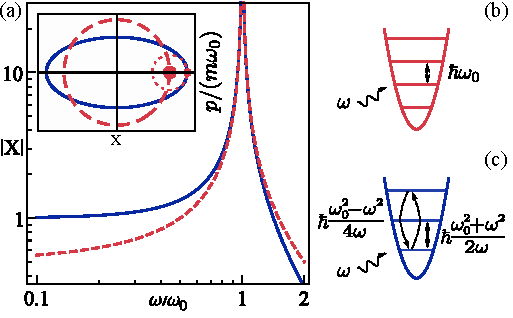
\includegraphics[width=0.75\textwidth]{figures/rwa/fig1.pdf}
	\caption{(a) Response amplitude [cf.~Eq.~\eqref{eq:exact_g}] of the driven harmonic oscillator as a function of the driving frequency $\omega$ for the exact solution (solid, blue) and the standard RWA solution (dashed, red) with $F_0=m=\omega_0=1$. The inset shows the corresponding phase space plots for large detuning, $\omega = 0.5$. Spheres indicate solutions in the rotating frame. The ansatz of stationary $\etil{a}$~(large red dashed circle) does not match the exact result. For this, an additional time-dependent term in the solution is needed~(small red circle). This term oscillates at $2\omega$, which results in an elliptical path.  (b) Energy quantization of the harmonic oscillator Hamiltonian~\eqref{eq:rot_H} with energy spacing $\hbar \omega_0$ using the operators $a,\,a^\dagger$ defined in Eq.~\eqref{eq:as}. (c) With the operators $b, b^\dagger$, the harmonic oscillator is not diagonalized, showing a level spacing of $\hbar (\omega_0^2+\omega^2)/ 2\omega$ and processes that create or annihilate two particles with amplitude $\hbar (\omega_0^2-\omega^2)/4\omega$.}
	\label{fig:fig1}
\end{figure}

Crucially, the response amplitude found with the RWA does not match the analytical solution in Eq.~\eqref{eq:exact_g}, see Fig.~\ref{fig:fig1}(a). Indeed, the ratio
\begin{equation}
\frac{x(t)}{x_{\text{RWA}}(t)} = \frac{2\omega_0\Delta}{\omega^2-\omega_0^2}= \frac{2\omega_0}{\omega_0+\omega}\,,
\end{equation}
only approaches unity for $\Delta \rightarrow 0$, which demonstrates the limitation of the RWA to near-resonant drives. 

A comparison  between the exact and RWA results in phase space is illustrative. To this end, we take a stationary amplitude $\etil{a} \equiv \abs{\etil{a}} $, and using Eq.~\eqref{eq:as}, we find the equivalent trajectory in phase space,
\begin{equation}
x(t) = 2\abs{\etil{a}} \sqrt{\frac{\hbar}{2 m \omega_0}} \cos(\omega t) \,, \quad p(t) = -2\abs{\etil{a}}\sqrt{\frac{\hbar m \omega_0}{2}} \sin(\omega t) \,.
\end{equation}
The resulting path is always circular, unlike the elliptical path of the exact solution, cf.~Eq.~\eqref{eq:exact_g} and Fig.~\ref{fig:fig1}(a).
Indeed, the dropped time-dependent oscillating terms, dubbed micromotion, add on to the circular path to produce the full elliptical motion, cf.~small circle in Fig.~1(a). This implies that to describe the elliptical path, $\etil{a}$ must be time-dependent, which cannot be obtained only by time-independent corrections from a high-frequency expansion~\cite{Mikami2016, Eckardt2017,Eckardt2015,Bukov2015,Goldman2014}.  
In other words, the assertion of a stationary $\etil{a}$ violates Hamilton's EOMs, specifically the relation $p = m \dot{x}$. This has also been described as a breakdown of the Ehrenfest theorem~\cite{Ford_1996}.

As the driven quantum harmonic oscillator is exactly solvable, the RWA was not necessary. Without the approximation, we would still have obtained the exact result. However, when the system becomes nonlinear, its EOMs are usually not exactly solvable. The RWA, being effectively the lowest order of a perturbative expansion, is then a common method to find the stationary response. As we have seen, however, it neglects crucial corrections due to the detuned drive frequency.
We identify that this systemic mismatch stems from the usual starting point~\eqref{eq:as}, which relies on operators that diagonalize the bare oscillator Hamiltonian and describe excitations with energies $\hbar \omega_0$, see Fig.\,\ref{fig:fig1}(b).

\subsection{RWA-adapted operator basis}
We now turn to our scheme for an exact treatment of the driven harmonic oscillator. We seek operators akin to $a$ and $a^\dagger$ which recover the ellipsoidal phase-space path corresponding to drive frequency $\omega$. A natural choice is to replace $\omega_0$ by $\omega$ in Eq.~\eqref{eq:as}, i.e., to define new operators $b$ and $b^\dagger$ via
\begin{equation} \label{eq:bs}
\hat{x} =\sqrt{\frac{\hbar}{2m\omega}}(b^\dagger+b)\,, \quad \hat{p} = i\sqrt{\frac{\hbar m \omega}{2}}(b^\dagger - b)\,,
\end{equation}
which satisfy $[b, b^\dagger]=1$, and describe the system in terms of excitations with the drive's frequency $\omega$. The driven harmonic oscillator Hamiltonian~\eqref{eq:qho} now reads
\begin{align} 
H = \hbar \bigg\{ &\frac{\omega_0^2 + \omega^2}{2 \omega}  \left (b^\dagger b + \frac{1}{2} \right)+ \frac{\omega_0^2  - \omega^2}{4 \omega} \big(b^2 + (b^\dagger)^2  \big)\nonumber
\\ &- F_b(e^{i\omega t} +e^{-i\omega t})(b^\dagger+b) \bigg\} \,,\label{eq:Hb}
\end{align}
with $F_b = F_0 / (2 \sqrt{2 m \omega \hbar})$, see Fig.~\ref{fig:fig1}(c). Note that we effectively rotated from the $a$ to the $b$ operators using a unitary (Bogoliubov) transformation~\cite{Xiao_2009}
\begin{equation}
%\begin{aligned}
%b &= \frac{1}{2} \left[ a \left(\sqrt{\frac{\omega_0}{\omega}} + \sqrt{\frac{\omega}{\omega_0}} \right)  + a^\dagger %\left(\sqrt{\frac{\omega_0}{\omega}} - \sqrt{\frac{\omega}{\omega_0}} \right)\right] \,,\\
%b^\dagger &= \frac{1}{2} \left[ a^\dagger \left(\sqrt{\frac{\omega_0}{\omega}} + \sqrt{\frac{\omega}{\omega_0}} \right)  + a %\left(\sqrt{\frac{\omega_0}{\omega}} - \sqrt{\frac{\omega}{\omega_0}} \right)\right] \,. \\
\mqty(a \\ a^\dagger) = \frac{1}{2} \mqty( \sqrt{\frac{\omega_0}{\omega}} + \sqrt{\frac{\omega}{\omega_0}} & \sqrt{\frac{\omega_0}{\omega}} - \sqrt{\frac{\omega}{\omega_0}} \\ \sqrt{\frac{\omega_0}{\omega}} - \sqrt{\frac{\omega}{\omega_0}} & \sqrt{\frac{\omega_0}{\omega}} + \sqrt{\frac{\omega}{\omega_0}}) \mqty(b \\ b^\dagger) \,.
%\end{aligned}
\end{equation}
With the new operators, Eq.~\eqref{eq:Hb} contains squeezing terms that do not conserve the particle number, since $b$ and $b^\dagger$ do not diagonalize the simple harmonic oscillator unless $\omega = \omega_0$. 

We repeat the RWA procedure in the new basis. We first apply the unitary transformation $U_b(t) = e^{-i \omega t b^\dagger b}$ to move to a rotating frame, and then obtain the corresponding Heisenberg's EOMs
\begin{equation} \label{eq:Heis_corr}
i \frac{d}{dt} \etil{b} = \frac{\omega_0^2 - \omega^2}{2\omega} \left( \etil{b} +  \langle \tilde{b}^\dagger \rangle e^{2 i \omega t}\right) - F_b\left(1  + e^{2 i \omega t} \right)\,.
\end{equation}
Crucially, when we now search for a stationary solution for $\etil{b}$, we obtain
\begin{equation}
\etil{b} = \frac{2F_b\,\omega}{\omega_0^2 - \omega^2} \,,
\label{eq:main_res}
\end{equation}
which upon inverting $U_b(t)$ matches the exact result in Eq.~\eqref{eq:exact_g}. Importantly, the correct result is obtained regardless of whether we take the RWA or not. In other words, when the operators $b, b^\dagger$ are used, the stationary solution in the rotating frame is exact and satisfies Eq.~\eqref{eq:Heis_corr}.

\subsection{Example: driven Duffing oscillator}
The RWA is a common starting point for dealing with time-dependent systems that are not exactly solvable. Our result~\eqref{eq:main_res} implies that a suitable choice of operators made prior to applying the RWA can significantly reduce errors at large detuning. To demonstrate this, we compare the results obtained using the RWA with the two operator definitions, $a,a^\dagger$ and $b,b^\dagger$. We consider a driven Duffing oscillator, described by the Hamiltonian
\begin{equation} \label{eq:H_Duffing}
H_D = p^2/2m + m \omega_0^2 x^2/2 + \alpha x^4/4 - F_0 \cos(\omega t)  x\,,
\end{equation}
where $\alpha$ is the Duffing nonlinearity. We plug both operator definitions [Eqs.~\eqref{eq:as} and~\eqref{eq:bs}] into Eq.~\eqref{eq:H_Duffing}, move to a rotating frame [Eq.~\eqref{eq:rot_H}], and apply the RWA in both procedures. Note that the RWA drops multiple oscillating terms that describe frequency conversion processes (see Sec.~\ref{sec:hb}) due to the Duffing nonlinearity. We furthermore apply a semiclassical mean-field ansatz\footnote{This means we take $\langle \tilde{a}^3 \rangle \rightarrow \etil{a}^3$ etc.} to obtain Heisenberg's EOMs
\begin{align} \label{eq:duff_a}
% 
i \frac{d}{dt} \etil{a} &=
% \Delta \etil{a} -F \left( 1 + e^{2i\omega t} \right) \\
% % + \frac{\alpha \hbar^2}{4 m^2 \omega_0^2} \Bigg(3\left\{\etil{a}+\etil{a^\dagger}e^{2i\omega t}\right\}\left[1+\etil{a}\etil{a^\dagger}\right]\\
% +\etil{a}^3e^{-2i\omega t}+\etil{a^\dagger}^3e^{4i\omega t}\Bigg)\\
% \xrightarrow[\mathrm{RWA}]{}
-\Delta \etil{a}-\frac{F_a}{\hbar}+\frac{3 \alpha \hbar}{4m^2\omega_0^2}\left(\etil{a}+\etil{a}^2\ave{\tilde{a}^\dagger}\right)\,,\\
\label{eq:duff_b}
i \frac{d}{dt} \etil{b} &= 
% \frac{\omega_0^2 - \omega^2}{2\omega} \left( \etil{b} +  \langle \tilde{b}^\dagger \rangle e^{2 i \omega t}\right) - F_b\left(1  + e^{2 i \omega t} \right) \\ 
% + \frac{\alpha h^2}{4 m^2\omega^2}  \Bigg(3\left\{\etil{b}+\etil{b^\dagger}e^{2i\omega t}\right\}\left[1+\etil{b}\etil{b^\dagger}\right]\\
% +\etil{b}^3e^{-2i\omega t t}+\etil{b^\dagger}^3e^{4i\omega t}\Bigg)\\
%  \xrightarrow[\mathrm{RWA}]{}
\frac{\omega_0^2 - \omega^2}{2\omega}\etil{b}-\frac{F_b}{\hbar}+\frac{3\alpha \hbar}{4m^2\omega^2}\left(\etil{b}+\etil{b}^2\ave{\tilde{b}^\dagger}\right)\,.
\end{align}

We can now search for stationary solutions in either of the rotating frames [$\frac{d}{dt} \etil{a} = 0$ or $\frac{d}{dt} \etil{b} = 0$]. Both Eqs.~\eqref{eq:duff_a} and~\eqref{eq:duff_b} generate a cubic polynomial condition which has up to three solutions (the B\'{e}zout bound, Sec.~\ref{sec:hb_solving}), see Fig.~\ref{fig:fig2}(a). Both approaches produce the expected tail-shaped response, i.e., a single solution in the $\omega < \omega_0$ regime that bends up towards a high-amplitude solution and a coexistence region in the $\omega > \omega_0$ regime, where both low- and high-amplitude solutions appear. 
%The latter resembles the coexistence of gas and liquid phases for cavity particles~\cite{ciuti, blatter}, and 
The coexistence region manifests mathematically as a bifurcation point for the roots of the polynomial condition. Despite the qualitative agreement, the solutions in the two frames differ quantitatively, i.e., in their amplitudes as a function of detuning and in the positions of their bifurcation points. 

\begin{figure}
	\centering
	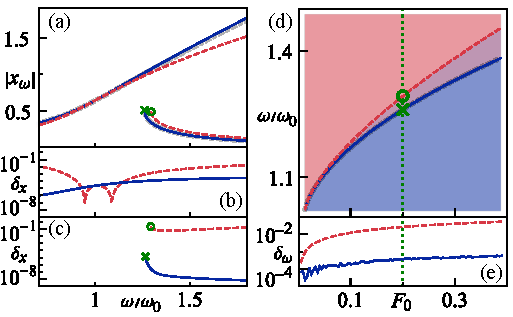
\includegraphics[width=0.75\textwidth]{figures/rwa/fig2.pdf}
	\caption{A comparison of the Duffing oscillator response obtained using the $a, a^\dagger$ and $b, b^\dagger$ operator bases [cf.~Eqs~\eqref{eq:as},~\eqref{eq:bs}] with a time-dependent simulation. The parameters used are $m=\omega_0=\alpha=1$. (a) The response amplitude $\abs{x_\omega}$ plotted against the drive frequency $\omega$ for $F_0=0.2$ using $a, a^\dagger$ (dashed, red) and $b,b^\dagger$ (solid, blue). The time-dependent simulation result (dot-dashed grey, behind blue) consists of adiabatic up and downsweeps of $\omega$.
		%The difference becomes more pronounced the larger the detuning $\Delta=\omega_0-\omega$. 
		(b), (c) The relative discrepancy in log scale of the $a,a^\dagger$ (dashed, red) and the $b, b^\dagger$ (solid, blue) results from the time-dependent simulation. %with the same log scale
		The circles and crosses in (a) and (c) represent the jump frequency in the downsweep for operators $a$ and $b$.
		%This jump corresponds to a phase transition of three unique solution to only one. 
		(d) A phase diagram as a function of $\omega$ and $F_0$. Blue (red) fill denotes regions with one (two) stable solution(s). %The adapted RWA (operator $b$) phase transition line in blue coincides well with the result of a time-dependent simulation (dot-dashed grey) but the standard RWA (operator $a$, dashed red) differs. The green dotted line indicates where the simulations (a-c) take place. 
		(e) Relative discrepancy $\delta_{\omega} = \abs{(\omega - \omega_{\text{RWA}}) \,/\, \omega }$ in log scale of the phase boundaries obtained using $a, a^\dagger$ (dashed, red) and $b, b^\dagger$ (solid, blue) from the time-dependent result. The phase boundaries were found with an $\omega$ resolution of $10^{-5}$, which becomes visible at low $F_0$, where the discrepancy of our scheme is of that order. The green dotted lines in (d) and (e) indicate where the simulation of (a) takes place.
	}
	\label{fig:fig2}
\end{figure}

To find out which of the two approximate procedures describes the driven Duffing oscillator~\eqref{eq:H_Duffing} more accurately, we compare their predictions with a ``numerical experiment'' in the classical picture. Specifically, we numerically evolve Hamilton's equations for the Hamiltonian~\eqref{eq:H_Duffing} until we reach stationary motion for different detunings and initial conditions and then adiabatically sweep the detuning to explore the solution landscape. Note that we add an infinitesimal dissipation term to enforce convergence in the simulation, which negligibly shifts the stationary outcome. 
Additionally, the numerical time-trace exhibits high harmonic generation -- this cannot be described by the RWA, regardless of which operators are used. Such limitation is not specific to the RWA, it is merely a result of using a single-harmonic ansatz (see Sec.~\ref{sec:hb}). Hence, the relevant benchmark for the RWA solutions is the Fourier component $x_\omega$ at frequency $\omega$ of the time trace. In Figs.~\ref{fig:fig2}(b) and (c), we plot the relative discrepancy $\delta_x = \abs{(x_\omega - x_{\omega, \text{RWA}})\, /\, x_\omega}$ between the numerically obtained $x_\omega$ and the two RWA results in the high- and low-amplitude solution branches, respectively. We observe that our new RWA approach agrees much better for all values of $\omega$. In the low-amplitude regimes, the system responds quasi-linearly and our scheme performs better as discussed above in the harmonic oscillator case. Slight deviations are seen in the high-amplitude regime, where nonlinear effects dominate the physics.

In driven-dissipative systems, phase diagrams depict the number or type of stationary solutions as a function of system parameters~\cite{Soriente_2018, Chitra_2015}. Here, we focus on the location of the bifurcation point as a function of detuning and drive amplitude.
%we commonly draw phase diagrams as a function of detuning and drive amplitude, where different regions mark a change in the number or type of stationary solutions~\cite{Soriente_2018, Chitra_2015}. 
The bifurcation point is marked in Figs.~\ref{fig:fig2}(a) and (c), where the better performance of our RWA approach manifests as a clear change in its position. In Fig.~\ref{fig:fig2}(d), we draw phase diagrams obtained by the two RWA approaches, and observe a distinct difference in the phase boundaries. The exact numerical solution matches our scheme much better, see Fig.~\ref{fig:fig2}(e).

\subsection{Discussion}
We have presented an operator basis for periodically-driven systems which anticipates a response at the driving frequency and is thus better suited for using the RWA. For both the harmonic and the Duffing oscillators, this basis choice significantly improves the fidelity of the RWA while retaining its simplicity. Our approach is applicable to systems in many areas of physics beyond mechanical oscillators described by $x$ and $p$~\cite{Bachtold_2022}. In quantum optics~\cite{Walls_Milburn} and optomechanics~\cite{Aspelmeyer_2014}, a driven cavity mode is described by Eq.~\eqref{eq:qho} with the magnetic and electric fields playing the roles of $x$ and $p$. For models with inherent detuning such as optomechanical cooling and frequency-comb generation, our approach may result in significant numerical corrections. Detuned driven systems also appear in circuit QED where the magnetic flux and charge appear in place of $x$ and $p$~\cite{Blais_2021}.

It is important to contrast the oscillator systems treated here to a driven two-level system. While the latter also gives inaccurate results when treated with the RWA, the root of the problem is different. Unlike the harmonic oscillator, a harmonically-driven two-level system displays many harmonics in its response~\cite{Zeuch_2020}, despite being linear. It is therefore impossible to correctly describe the response using a single-harmonic ansatz such as that employed in Eq.~\eqref{eq:exact_g}. A specific case of interest are models coupling a cavity to one or more two-level systems~\cite{Shore_1993,Kirton_2019}; here the so-called general RWA is used, where a basis diagonalizing the spin-cavity interaction reduces the RWA error~\cite{Irish_2007}. As general RWA uses the standard operators $a$ and $a^\dagger$, we expect that it can be improved further by using our scheme. 

Overall, a sizeable body of work exists elaborating on the errors due to the RWA at large detuning~\cite{Baker_2018, Niemczyk_2010, Bishop_2010, Sornborger_2004}. Our work suggests that in many cases, these errors can be dramatically reduced by choosing an appropriate operator basis. The errors are partially due to the RWA assuming a single-frequency response, which cannot describe strongly nonlinear behaviour Nevertheless, as we show in this work, the standard RWA already fails to describe a single-frequency response if the system is driven off-resonantly. Using the suggested operator definition fixes this problem, and reduces the RWA errors to those truly inherent to the single-harmonic description.

\section{General harmonic ansatz for quantised variables} \label{sec:rwa_gen}

To complete the integration of quantised variables into our harmonic balance framework, we extend the operator basis found in Eq.~\eqref{eq:bs} to formulate a general harmonic ansatz, similar to Eq.~\eqref{eq:hb_ansatz_a}. For a system of $N$ pairs of conjugate variables, $\hat{x}_j$ and $\hat{p}_j$, we seek an expansion in terms of \textit{harmonic operators} $b_{j,k} ,\, b_{j,k}^\dagger$, with the requirement that
\begin{equation}
\begin{aligned}
&[b_{j,k} , \, b_{j'k'}^\dagger ] = \delta_{jj'} \delta_{kk'} \,, \quad  \left[\hat{x}_j , \, \hat{p}_{j'} \right ] = \delta_{jj'} i \hbar \\
&\left[b_{j,k} , \, b_{j'k'} \right] = \left[\hat{x}_j , \, \hat{x}_{j'} \right ] = \left[ \hat{p}_j ,\, \hat{p}_{j'} \right] = 0 
\end{aligned}
\end{equation}
The desired formulation involves renormalizing all harmonic operators by the number of harmonics present, $K$,
\begin{equation} \label{eq:rwa_general_ansatz}
\begin{aligned}
\hat{x}_j &= \sqrt{\frac{\hbar}{2mK}} \sum_{k=1}^K \sqrt{\frac{1}{\omega_k}} \left( b_{j,k} \e^{i \omega_k t} + b_{j,k}^{\dagger} \e^{-i \omega_{k} t} \right) \,, \\
\hat{p}_j &= i\sqrt{\frac{\hbar m}{2K} } \sum_{k=1}^K \sqrt{\omega_k} \left(b_{j,k} \e^{i \omega_k t} - b_{j,k}^{\dagger} \e^{-i \omega_{k} t} \right) \,.
\end{aligned}
\end{equation}
Note that this procedure very much resembles a standard textbook quantisation of systems such as an optical cavity~\cite{Walls_Milburn}. We stress again that standard quantisation focuses on the solutions of a conservative system -- its normal modes. Each mode possesses a natural frequency, which would be observed under energy-conserving time evolution from an initial condition. In a driven-dissipative system, however, the normal mode frequencies do not play any special role in the formalism. They are merely one of the underlying parameters. For steady states to be consistent with Hamilton's equations, the harmonics $\omega_k$, fixed by the drive, must be used for the second quantisation instead.

\subsubsection{Velocity-dependent potentials}

Finally, we remark that the relations between $\hat{x}$ and $\hat{p}$ imposed throughout this Chapter rely on the Ehrenfest theorem, $m \hspace*{0.3mm} d \hspace*{-0.6mm} \expval{\hat{x}} / dt = \expval{\hat{p}}$. This however assumes a velocity-independent potential. Where that is not the case, the general Ehrenfest theorem for a Hamiltonian $H$,
\begin{equation}
\frac{d }{dt} \expval{\hat{x}_j}= \frac{1}{i \hbar} \expval{\left[\hat{x}_j, H \right]} + \expval{\frac{\partial \hat{x}_j}{\partial t}}\,,
\end{equation}
must be used to construct a suitable harmonic ansatz. 